\section{Menus}
\ourgame{} has three menus: the \textbf{Main Menu}, which is displayed to the user when the game is launched and when the user pauses the game; the \textbf{Options Menu}, which can be accessed through the Main Menu; and the \textbf{Inventory Menu}, which can be accessed during gameplay. 

\begin{figure}[htb]
  \centering\begin{subfigure}{.33\textwidth}
    \centering
    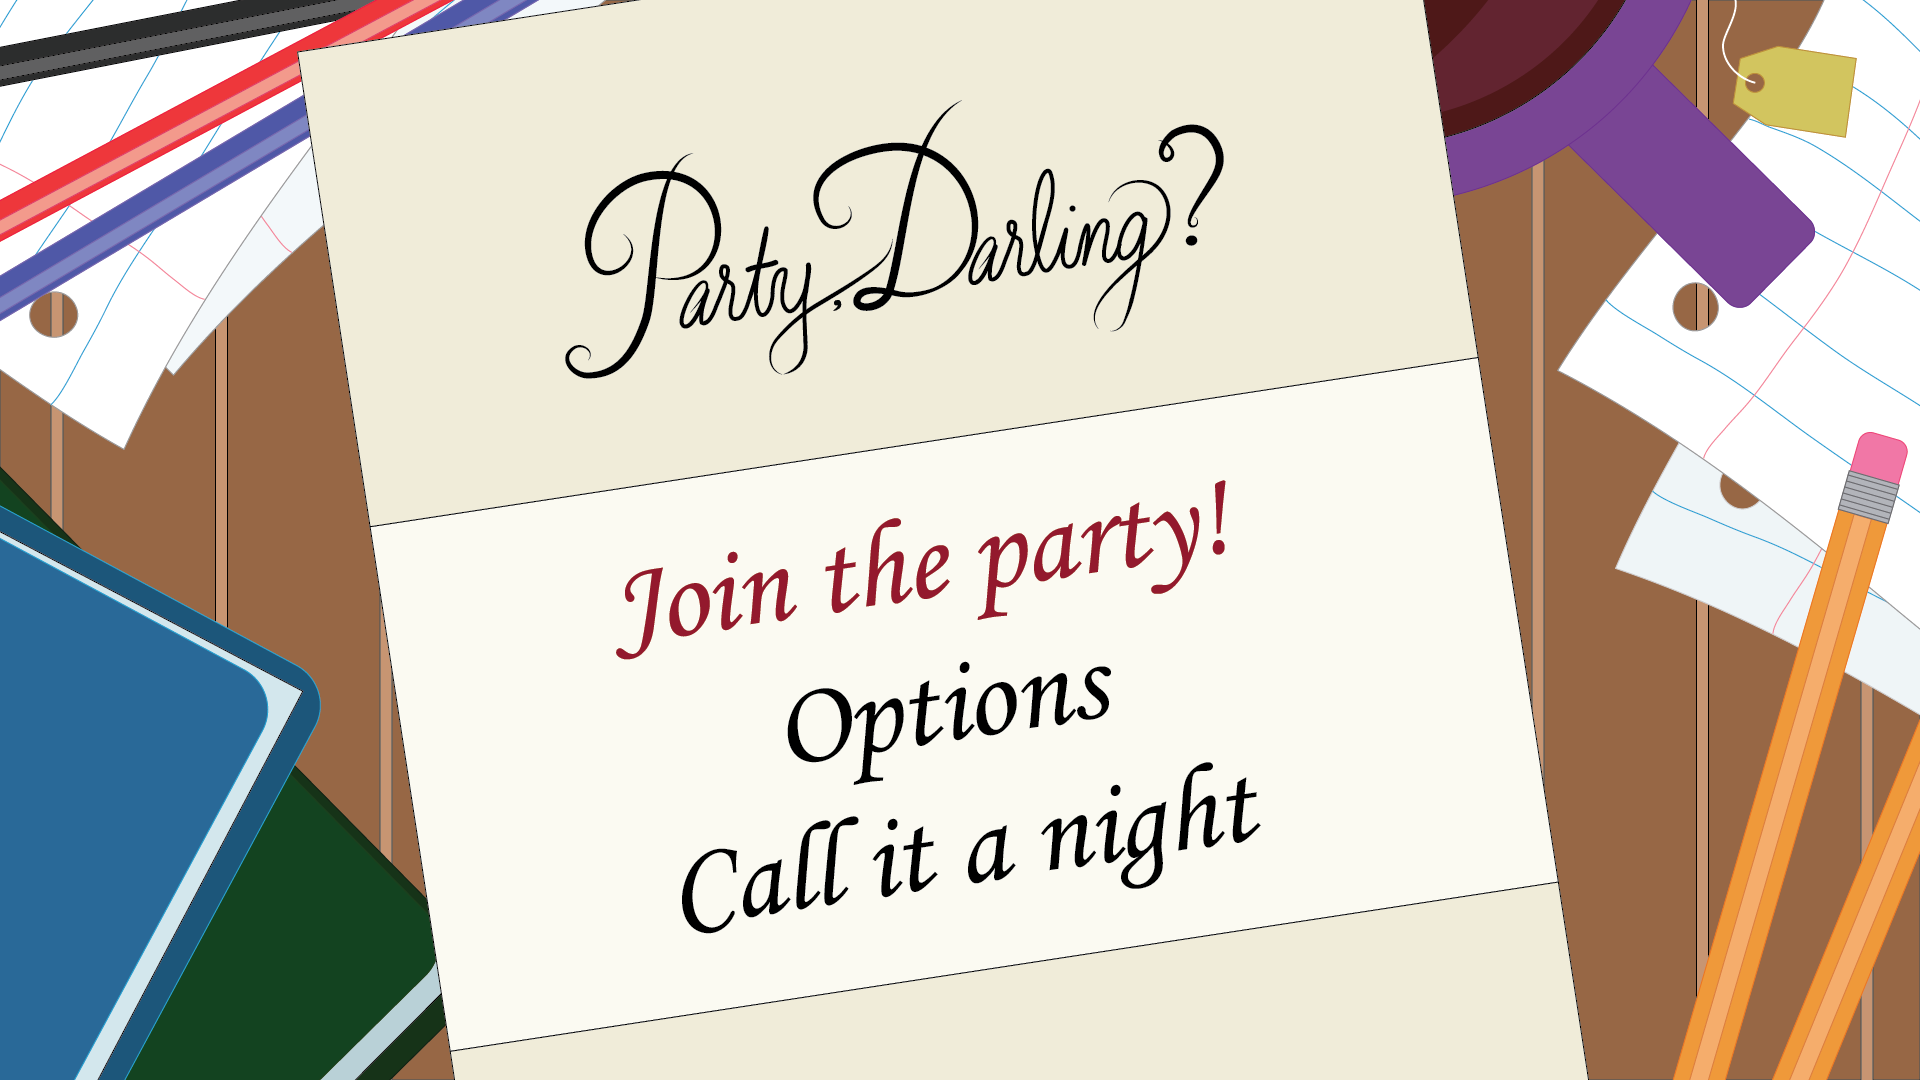
\includegraphics[width=.9\linewidth]{images/menu_main}
    \caption{Main Menu}
    \label{fig:menu_main}
  \end{subfigure}
  \begin{subfigure}{.33\textwidth}
    \centering
    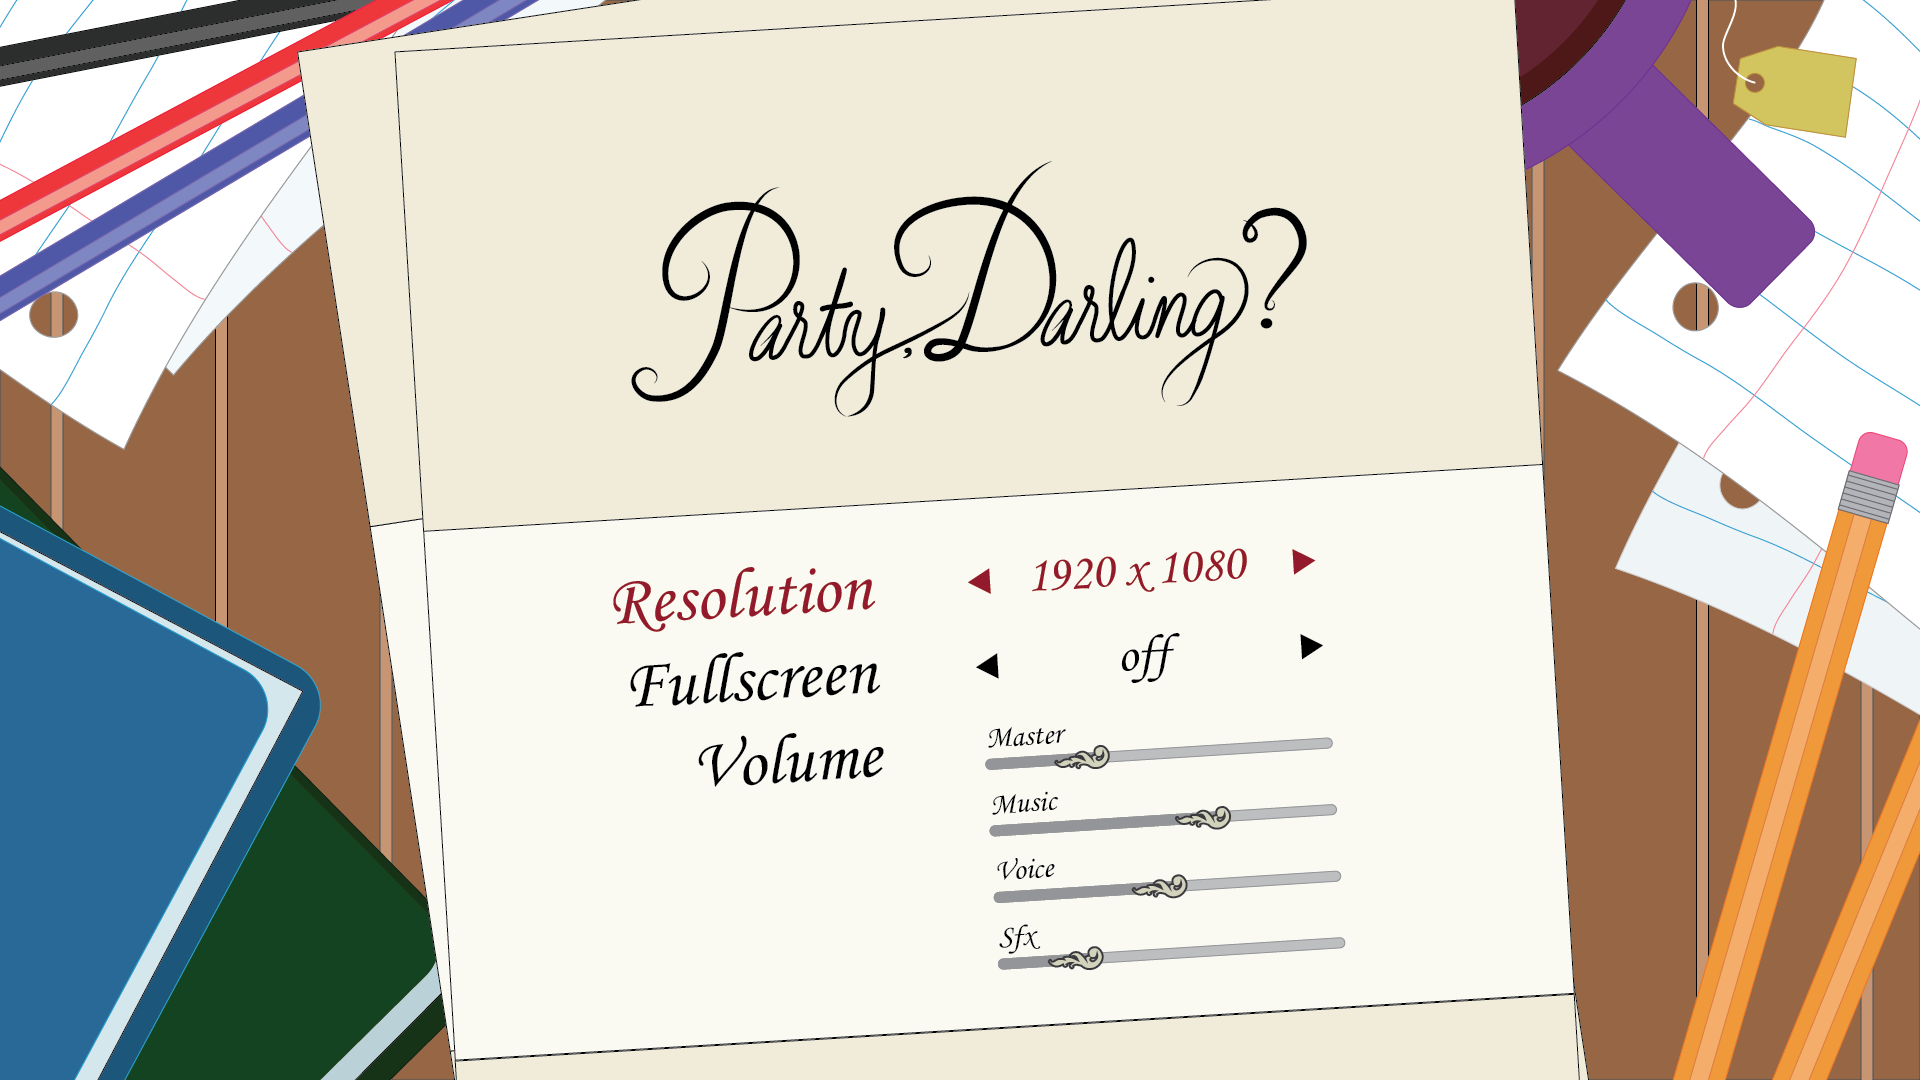
\includegraphics[width=.9\linewidth]{images/menu_options}
    \caption{Options Menu}
    \label{fig:menu_options}
  \end{subfigure}
  \begin{subfigure}{.33\textwidth}
    \centering
    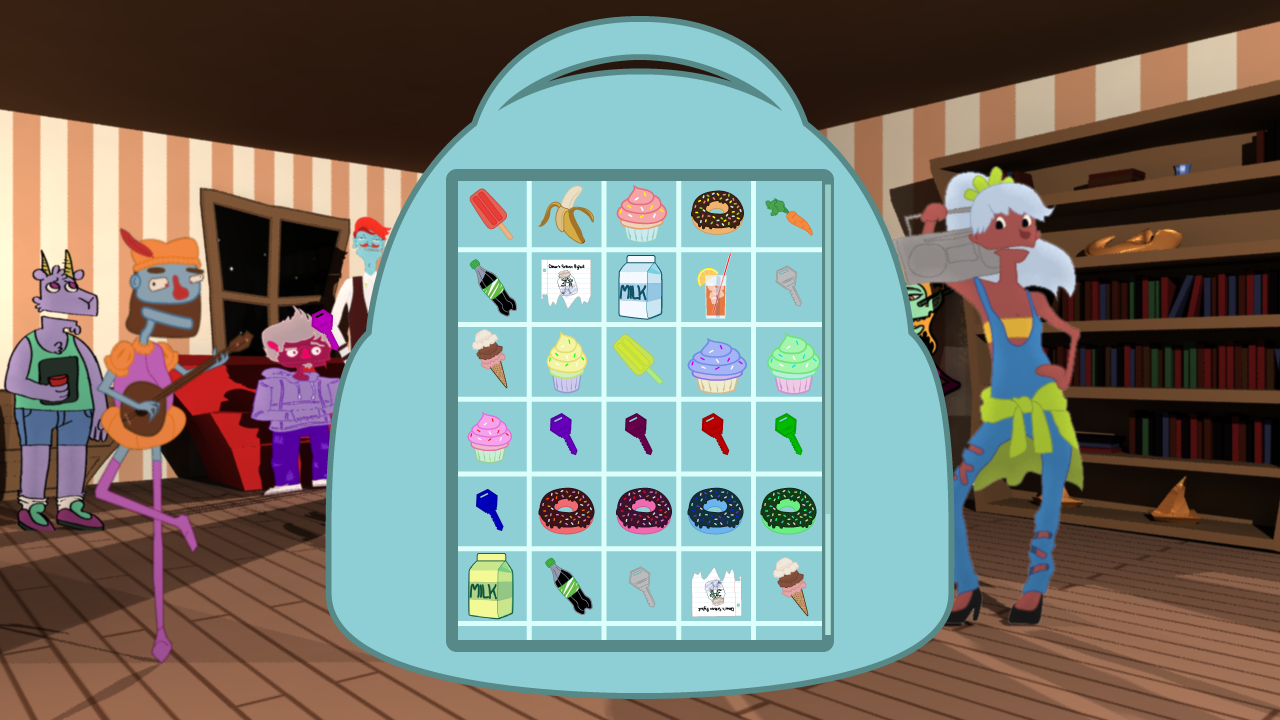
\includegraphics[width=.9\linewidth]{images/grid1}
    \caption{Inventory Menu}
    \label{fig:menu_inventory}
  \end{subfigure}
  \caption{Menus in \ourgame{}}
  \label{fig:menus}
\end{figure}

\subsection{Main Menu}
The main menu of \ourgame{} will include three main options:
\begin{enumerate}
\item{Join the party!: Start a new game, or continue a previously saved game}
\item{Options: Configure the game's settings}
\item{Call it a night: Prompts the user to quit the game}
\end{enumerate}

\subsection{Options Menu}
The options menu of \ourgame{} will include three main controls, one of which is split into four sub-controls: 
\begin{enumerate}
\item{Resolution: Sets the game window size to one of the monitor's supported video modes}
\item{Fullscreen: Lets the user decide whether to run the game in windowed or fullscreen mode}
\item{Categorized volume controls: Lets the user decide the volume of different elements of the game individually
\begin{enumerate}
	\item{Master: affects the volume of every audio file played}
	\item{Music: affects the volume of the audio files containing background music}
	\item{Voice: affects the volume of the audio files used when characters are speaking}
	\item{Sound Effects: affects the volume of the rest of the audio files used throughout the game}
\end{enumerate}}
\end{enumerate}

\subsection{Inventory Menu}
\label{sec:inventory}
As players will typically come across many different items in a single run, \ourgame{} will have an inventory system which allows the player to store these items for later use. This inventory will show all of the player's currently stored items as 2D sprites inside a backpack's outline. Items will be organized within a grid, where identical items stack and are represented by a single sprite within the inventory. An infinite number of items can be added to the inventory, with items received most recently appearing in the most bottom-right cell of the grid. To navigate within the inventory, the user can either move the navigation bar on the right side of the user interface, or spin the scroll wheel. The player can learn more information about an item, including its name, description, quantity, and effect, by hovering over the item's sprite causing a pop-up with the information to appear. If the user clicks on an item, it will be selected and the screen will change to show the options the user has, as can be seen in Figure~\ref{fig:UI_item}.

\begin{figure}[htb]
\centering
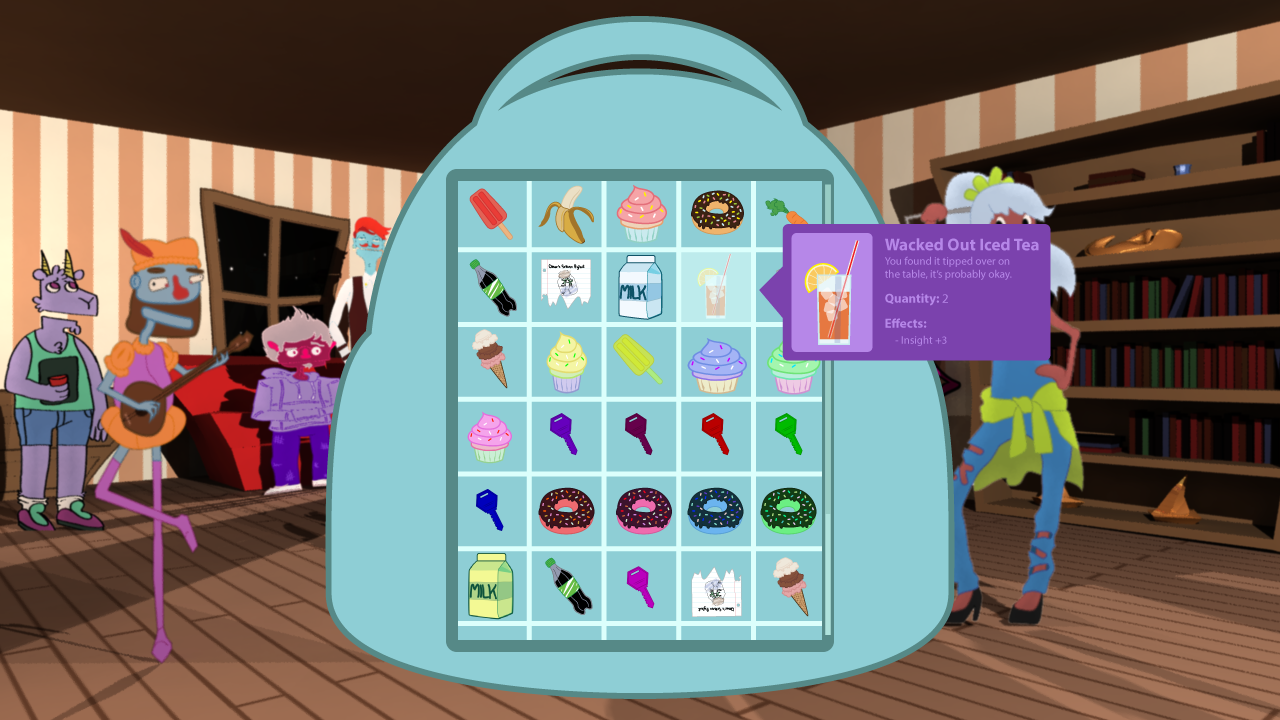
\includegraphics[width=.6\linewidth]{images/grid_Hovered}
\caption{Inventory item info pop-up}
\label{fig:inventory_grid_hovered}
\end{figure}
